% IEEE journal format (IEEEtran). References count toward the page total.
\documentclass[journal]{IEEEtran}

% Math
\usepackage{amsmath,amssymb,mathtools}

% Typography
\usepackage[utf8]{inputenc}
\usepackage[T1]{fontenc}
\usepackage{url}
\usepackage{booktabs}
\usepackage{microtype}
\usepackage{xcolor}
\usepackage{graphicx}
\usepackage{cite}

% hyperref before cleveref
\usepackage[hidelinks]{hyperref}
\usepackage[capitalize,noabbrev]{cleveref}
\crefname{figure}{Fig.}{Figs.}
\Crefname{figure}{Fig.}{Figs.}
\crefname{table}{Table}{Tables}
\Crefname{table}{Table}{Tables}
\crefname{section}{Section}{Sections}
\Crefname{section}{Section}{Sections}
\crefname{subsection}{Section}{Sections}
\Crefname{subsection}{Section}{Sections}
\crefname{appendix}{Appendix}{Appendices}
\Crefname{appendix}{Appendix}{Appendices}

% math_commands.tex: notation shared across sections
\newcommand{\vmu}{\boldsymbol{\mu}}
\newcommand{\mSigma}{\boldsymbol{\Sigma}}
\newcommand{\mI}{\mathbf{I}}
\newcommand{\kap}{\kappa}      % shrinkage strength of the hybrid


\title{How Much Personal History Is Enough? Measuring the Data Requirement for Individualised Financial Behavioural Anomaly Detection}

\author{Briyan~George~Dyju%
\thanks{B.~G.~Dyju is an independent researcher in Dubai, United Arab Emirates (e-mail: briyandyju@gmail.com).}}

\begin{document}

\maketitle

\begin{abstract}
Detecting unusual financial behaviour by comparing a transaction with a person's own history raises a question that deployed systems settle by fiat: how many transactions make a personal baseline worth using? We measure it. Data-efficiency curves for six unsupervised detectors, evaluated on 300 real bank accounts, a 240-person controlled simulation and 300 entities of a synthetic card dataset, show that a shrinkage-regularised Mahalanobis detector reaches 90\% of its best ranking performance (precision-recall AUC 0.657) at 25 personal transactions and gains nothing measurable beyond 100; the threshold is identical across five independent cohort draws. Labels come from provenance, not from any detector: a held-out transaction is replaced by a real transaction from a different account. Below about 10 transactions a population model outperforms personalisation, and a history-weighted shrinkage hybrid removes that penalty at no measurable cost later. Operating-point behaviour depends on how the alert threshold is calibrated: scoring the model's own training data makes the detector flag 96\% of transactions at 10 personal transactions, whereas leave-one-out calibration leaves it nearly silent there (1.2\%) and close to its nominal false-positive rate from 25. Detector rankings under scarcity reverse between datasets, and behavioural variability predicts the requirement under controlled manipulation (Spearman correlation 0.48 to 0.71) but not across real accounts. An anomaly here is a deviation from a baseline, not fraud.

\end{abstract}

\begin{IEEEkeywords}
anomaly detection, personalisation, cold start, learning curves, transaction data, threshold calibration
\end{IEEEkeywords}

\section{Introduction}\label{sec:intro}

A personalised anomaly detector compares each new transaction with a model of one person's own past behaviour. The appeal is plain: a 900-unit purchase is unremarkable for one account holder and extraordinary for another, and a single population-wide rule serves both badly.

The approach carries an equally plain dependency. The personal model has to be estimated from the person's own transactions, and when an account opens there are none. Somewhere between zero transactions and a lifetime of them, the personal baseline becomes worth using. Production systems settle the question with a cutoff; one patent family describes filtering out ``unseasoned users, i.e.\ users with insufficient history'' \cite{faigon2021anomaly}. The cutoff is treated as a known engineering parameter, yet we found no published measurement of where it lies or whether it exists (\cref{sec:related}).

We measure it. For each account we hold a 60-transaction evaluation window fixed and train on the $n$ transactions immediately preceding it, with $n$ from 1 to 250 on real data and to 500 on synthetic data, so that every comparison across history sizes is paired at the account level. Anomalies are defined by provenance: a held-out transaction is replaced by a real transaction from a different account, so no detector's score can define its own labels. We run six unsupervised detectors on 300 accounts of the PKDD'99 Berka bank data, on a controlled simulation of 240 individuals whose variability we set directly, and on 300 card entities of IBM's synthetic TabFormer data, which carries merchant, category and geographic channels that Berka lacks.

The shape of the answer is an early plateau. A shrinkage-regularised Mahalanobis detector reaches 90\% of its best precision-recall AUC (PR-AUC, 0.657 against a 0.10 prevalence baseline) at 25 personal transactions, and the threshold is 25 at each of five independent cohort draws. The single number conceals three dependencies that the rest of the paper quantifies: the threshold moves with the detector and the dataset, the usable alert threshold moves with the calibration rule, and below the sufficiency point a population model beats the person's own history.

\paragraph*{Contributions}
\begin{enumerate}
\item \textbf{A measured sufficiency point.} Data-efficiency curves for per-user anomaly detection under a provenance-labelled, paired protocol. On Berka, Mahalanobis distance reaches 90\% of its best PR-AUC at 25 personal transactions and gains nothing measurable beyond 100; the same early-plateau shape appears on TabFormer, with a threshold of 250 (\cref{sec:curves,sec:tabformer}).
\item \textbf{A crossover and its remedy.} A population model outperforms the personal model below about 10 transactions for Mahalanobis and 50 for $k$-NN on Berka. A history-weighted shrinkage hybrid is never meaningfully worse than either parent at any size on Berka and removes the cold-start penalty without a measurable cost at large $n$ (\cref{sec:arms}).
\item \textbf{A calibration effect that changes the operating point.} Calibrating the alert threshold on the model's own training scores makes Mahalanobis flag 96\% of transactions at $n=10$; leave-one-out (LOO) calibration makes it flag 1.2\% there and brings the false-positive rate within 1.6 to 3 points of the nominal 5\% from $n=25$. The effect holds across six detectors and five seeds, and it does not always push in the same direction (\cref{sec:calibration}).
\item \textbf{The limits of transfer.} Detector rankings under scarcity reverse between datasets (Isolation Forest is weakest on Berka and strongest at small $n$ on TabFormer); behavioural variability predicts the requirement under controlled manipulation (Spearman $\rho=0.48$ to $0.71$) but not across real accounts; and a direct drift measurement rules out drift as the explanation for the negative marginal gain from 100 to 250 transactions (\cref{sec:variability,sec:recency,sec:tabformer}).
\end{enumerate}

\Cref{sec:related} positions the work, \cref{sec:setting} defines the setting and data, \cref{sec:protocol} the protocol, and \cref{sec:results} reports results. \Cref{sec:discussion} draws out what the evidence establishes and \cref{sec:limits,sec:ethics} give limitations and ethical considerations.

\section{Related Work}\label{sec:related}

\paragraph{Behavioural profiling for card fraud}
Per-user profiling for card fraud is mature. Dal~Pozzolo \emph{et al.}\ formalise realistic evaluation, including feature augmentation from cardholder profiles and the interaction between alerts and investigator feedback \cite{dalpozzolo2018realistic}, and report lessons learned from a practitioner perspective \cite{dalpozzolo2014learned}. Correa~Bahnsen \emph{et al.}\ aggregate raw transactions into spending-behaviour features per cardholder \cite{bahnsen2016feature}. Jurgovsky \emph{et al.}\ treat detection as sequence classification over a card's transaction stream \cite{jurgovsky2018sequence}, and Lucas and Jurgovsky survey the field's recurring problems of class imbalance, dataset shift and evolving behaviour \cite{lucas2020survey}. These works build and evaluate personal models; none asks how much personal history the model needs.

\paragraph{Personal baselines in deployed systems}
Granted patents describe personal-baseline methods directly. One family builds per-user profiles from the median, the median absolute deviation and a ``median of abnormality'' statistic, and scores new activity by its relative deviation \cite{saunders2021profile,saunders2023profile}. Another constructs separate per-user models and explicitly filters out users with insufficient history \cite{faigon2021anomaly}. Both treat the sufficiency cutoff as a given; we measure it.

\paragraph{Cold start}
Graph-based methods such as SparseFraudNet address users with thin histories through relational aggregation over other accounts \cite{zhang2025sparsefraudnet}. This routes around the per-user data requirement rather than quantifying it.

\paragraph{Learning curves}
Viering and Loog review the shapes of learning curves and establish that no universal functional form exists: curves are commonly power-law or exponential but can be ill-behaved, and both rate and saturation level are task-dependent \cite{viering2023shape}. Mohr and van Rijn survey their use in decision making \cite{mohr2022learning}. Per-user cold-start sweeps appear in recommender systems, where SPMC caps per-user interaction counts and reports performance across the cap \cite{cai2017spmc}. We apply this toolkit to the question the fraud literature leaves open.

\paragraph{Gap}
The field knows how to build personal behavioural models, knows that thin histories are a problem, and has general tooling for performance against training-set size. We found no study that reports, for unsupervised behavioural anomaly detection on financial transactions, performance as a function of the number of transactions in the individual's own history, with an operational sufficiency criterion and a matched comparison against population and hybrid models at each size. The search used open web sources; paywalled venues were reachable only through abstracts and citing-paper summaries, so the gap stands as the result of a documented search, not a proof of absence.

\section{Problem Setting and Data}\label{sec:setting}

\subsection{Setting}
An \emph{entity} is an account (Berka) or a (user, card) pair (TabFormer). The \emph{personal history size} $n$ is the number of the entity's own transactions available to fit a detector, taken from immediately before the evaluation window (\cref{sec:protocol}). A detector is unsupervised: it sees only the entity's past transactions, never labels.

We use \emph{behavioural anomaly} for a transaction that deviates from a pattern established by prior observations of the same entity. Behavioural anomalies, statistical outliers, suspicious transactions and confirmed fraud form no implication chain: a statistical outlier is a model artefact, a suspicious transaction is an institutional judgement involving policy and cost, and confirmed fraud requires evidence external to the transaction record. Most behavioural anomalies are benign (a holiday, a house move, a new job). A detector of behavioural anomalies identifies deviations from a baseline; it does not establish fraud or wrongdoing, and nothing in our labels is fraud.

We ask six questions. How does detection performance grow with $n$, and where does it saturate? Can a defensible sufficiency threshold be identified, and do different definitions of it agree? Does the requirement depend on the individual's behavioural variability? Is transaction count or temporal coverage the binding constraint? How do personal, population and hybrid models compare at each $n$? Do sophisticated detectors beat simple statistics under scarcity?

\subsection{Real Bank Data: PKDD'99 Berka}
The PKDD'99 Financial dataset \cite{berka1999pkdd} holds real, anonymised retail-banking transactions from a Czech bank: 1{,}056{,}320 transactions across 4{,}500 accounts from 1993-01-01 to 1998-12-31. Per-account depth has median 208, mean 234.7 and maximum 675; 3{,}883 accounts have at least 100 transactions, 1{,}835 at least 250 and 119 at least 500. Each transaction carries a date (day resolution), a credit/debit type, one of five operation modes, an amount, a balance, one of seven characterisation symbols (\texttt{k\_symbol}) and partner bank and account fields. The data have no fraud or anomaly labels.

Berka is the only real dataset we assessed that satisfies the requirements of per-entity identity, timestamps, sufficient per-entity depth and real behaviour. The most-cited card dataset (ULB) lacks a cardholder identifier, which makes per-user histories impossible; the IEEE-CIS competition data carry no entity key beyond a reverse-engineered competition artefact; and the remaining candidates (Sparkov, PaySim, BankSim, IBM AML) are synthetic with shallow per-entity histories or network-level tasks, while Bank Account Fraud contains application records rather than transaction sequences.

The primary host did not resolve from our execution environment, so files came from a GitHub mirror. The loader checks every one of the eight tables against the record counts published on the primary page and raises on mismatch; all eight matched. We additionally cross-checked every table byte-for-byte, after line-ending normalisation, against a second independent mirror; the SHA-256 digests are in the repository's data-integrity report. The data are released for an open research challenge and carry no machine-readable licence; we use them for research only and redistribute no raw records.

\subsection{Synthetic Card Data: TabFormer}
IBM's TabFormer credit-card dataset \cite{padhi2021tabular} is generator-produced, not real behaviour, so we never pool it with Berka or with the behavioural simulation. We use it for one narrow purpose: to test whether the curve shape found on one 1990s retail-banking dataset reappears on a schema with merchant, category, geographic and minute-resolution timing channels. It holds 24{,}386{,}900 transactions from 2{,}000 users, independently counted by a full chunked pass over the downloaded file. The entity is a (user, card) pair, because a person can hold several cards with materially different usage; 6{,}139 distinct pairs exist and 4{,}538 have at least 560 transactions. We use amount, chip use (swipe, chip or online), merchant name, merchant city and state, merchant category code (109 distinct values), the error field and time to the minute, plus the generator's own fraud label (0.122\% prevalence). Only the primary GitHub LFS endpoint was downloaded, so provenance is weaker than Berka's two-mirror check.

\subsection{Controlled Simulation}
The real data cannot supply merchant, category or geographic channels, nor \emph{controlled} variability. We therefore simulate 240 individuals across six archetypes of 40 each. Each individual is defined by a measurable parameter vector rather than a label: log-amount dispersion, merchant count and Zipf exponent, category count, location count and home-location weight, inter-arrival Gamma shape, hour-of-day von Mises concentration, and a drift rate that rotates merchant and category distributions over time. The archetypes are \emph{regular} (log-amount dispersion 0.30, 5 merchants, 1 location), \emph{moderate}, \emph{variable} (dispersion 1.10, 60 merchants, 8 locations), \emph{traveller} (15 locations, home weight 0.35), \emph{seasonal} (drift rate 0.004) and \emph{burst} (Gamma shape 0.35, producing inactivity punctuated by clusters). Anomalies fall into six classes (amount, merchant, category, geographic, temporal and multivariate), each generated from a deliberately shifted distribution independent of any detector; ground truth is the generating branch, which no detector observes. Simulation results are never pooled with real-data results.

\section{Experimental Protocol}\label{sec:protocol}

\subsection{Split Design}
For each entity, the \emph{evaluation window} is its last 60 transactions (100 in the simulation), and the training history of size $n$ is the $n$ transactions immediately preceding that window:
\begin{equation*}
[\;\text{earlier history}\;\mid\;\underbrace{n\ \text{training}}_{\text{varies}}\;\mid\;\underbrace{60\ \text{evaluation}}_{\text{fixed}}\;].
\end{equation*}
No transaction is ever both trained on and tested on, at any $n$. Because the window is identical across $n$ for a given entity, comparisons across history sizes are paired at the entity level, and differences in window difficulty between entities cancel in paired tests. The population (global) model is fitted on the \emph{earliest} transactions of donor entities that are disjoint from the evaluated entities, so it never sees an evaluated entity's data and is not advantaged by seeing later data.

On Berka we evaluate $n\in\{1,5,10,25,50,100,250\}$ on one fixed cohort of accounts with at least 310 transactions (1{,}319 eligible; 300 evaluated and 400 donors). Extending to $n=500$ needs 560 transactions per account, which about 60 of the most active accounts have; the $n=500$ point would be computed on a biased cohort a fifth the size of every other point and would break the pairing. The simulation and TabFormer, where depth is not a constraint, extend to $n=500$ (TabFormer: 300 evaluated and 400 donor entities; eligibility requires at least 560 transactions).

\subsection{Ground Truth}
Labelling anomalies with a statistical rule and then evaluating detectors that compute something similar measures agreement between two versions of one rule. We avoid this circularity.

\paragraph{Protocol I (primary): impostor substitution}
A held-out transaction of the target entity is replaced by a real transaction from a different real entity. The replacement keeps the target's timeline slot and takes the impostor's amount, type, operation and \texttt{k\_symbol}. Ground truth is provenance: a different person's real behaviour produced the row, and no statistical criterion is involved. Substitution replaces insertion because insertion would perturb the surrounding inter-arrival gaps and let detectors exploit that artefact instead of behaviour. As a consequence, timing carries no discriminative signal under Protocol I, since the injected row inherits the target's true date.

\paragraph{Protocol P (secondary): parametric perturbation}
A held-out transaction is replaced by a copy of itself with its amount multiplied by 5.

Injection rate is 10\% in both protocols, giving six anomalies per 60-transaction window. Injection is performed once per entity and shared across all history sizes, which preserves the pairing.

\subsection{Features}
Berka features have 21 dimensions and depend only on the transaction and strictly earlier transactions of the same account: log amount; a credit indicator; day-of-month and day-of-week as sine and cosine pairs; log inter-arrival gap; one-hot operation (5 plus missing); and one-hot \texttt{k\_symbol} (7 plus missing). The account balance is excluded: it is accumulated state, not a behavioural choice, and under Protocol I a substituted row would carry a balance discontinuity that reveals provenance without reflecting behaviour. TabFormer features have 26 dimensions (13 numeric or binary plus a 13-level merchant-category-code one-hot). Standardisation is fitted on training history only. At $n=1$ dispersion is undefined and scales collapse to unity; we record this as a degenerate regime.

\subsection{Detectors}
\begin{itemize}
\item \textbf{Gaussian z} and \textbf{robust z}: $|z|$ of log amount using mean and standard deviation, or median and median absolute deviation.
\item \textbf{Mahalanobis}: Mahalanobis distance from the training mean under a shrinkage-regularised, ridge-stabilised covariance estimate.
\item \textbf{$k$-NN}: distance to the fifth nearest training point. With $n$ from 1 to 25 in a 21-dimensional, one-hot-heavy space, cluster counts and density parameters for $K$-means or DBSCAN cannot be estimated without tuning on data we do not have. Distance to the $k$th neighbour belongs to the same family of density-based methods as LOF \cite{breunig2000lof}, needs no cluster count and degrades gracefully.
\item \textbf{Isolation Forest} \cite{liu2008isolation}: 200 trees, seeded, with subsample size $\min(256,n)$ (scikit-learn \cite{pedregosa2011scikit}).
\item \textbf{Autoencoder}: a $d$-4-$d$ network with tanh units ($d=21$ on Berka, $d=26$ on TabFormer), full-batch Adam (learning rate 0.01, weight decay $10^{-4}$, 300 epochs), implemented in NumPy.
\end{itemize}

\paragraph{Shrinkage hybrid}
The hybrid shrinks personal location and scatter toward population estimates with a weight determined solely by $n$:
\begin{align}
\vmu_{h} &= \frac{n\,\vmu_{p}+\kap\,\vmu_{g}}{n+\kap}, &
\mSigma_{h} &= \frac{n\,\mSigma_{p}+\kap\,\mSigma_{g}}{n+\kap}+\epsilon\mI,
\end{align}
where subscripts $p$ and $g$ denote personal and global estimates, $\epsilon\mI$ is a small ridge term, and $\kap=25$ is fixed in advance, not tuned on test data. At $n=0$ the hybrid is exactly the global model; as $n$ grows it converges to the personal model.

\subsection{Evaluation}
At 10\% prevalence a detector that flags nothing scores 90\% accuracy while detecting nothing, and accuracy changes with prevalence without any change in the detector. We therefore report precision-recall AUC (PR-AUC) as the primary metric, since both precision and recall condition on the minority class \cite{saito2015precision}, and the prevalence baseline is 0.10.

\paragraph{Operating point and calibration rules}
Operating-point metrics (flag rate, false-positive rate (FPR), recall, precision) need an alert threshold, and choosing one on test labels would leak. We set the threshold at the 95th percentile of training scores, so the nominal FPR is 0.05, and compare two ways of obtaining those scores. The \emph{in-sample} rule scores each training point with the model fitted on all $n$ training points. The \emph{leave-one-out (LOO)} rule scores each training point with a model fitted on the other $n-1$ points (exact refits, no approximation); it is undefined at $n=1$, where the rule flags nothing. Both rules are computable by a deployed system.

\paragraph{Sufficiency thresholds}
We apply three operational definitions to the same mean curves over the evaluated grid. The \emph{relative-$q$ threshold} is the smallest evaluated $n$ whose mean PR-AUC reaches $q\%$ of the curve's best observed value and is never later undercut; we use $q=90$ and report $q=95$. The \emph{stability threshold} is the smallest $n$ from which the across-account standard deviation of PR-AUC stays at or below the median of that model's own standard deviations over all sizes. An \emph{absolute} threshold needs a policy level that should follow from the cost of a false positive in a deployment we do not model, so we do not set one. Saturation is also fitted as $y(n)=y_{\max}-(y_{\max}-y_0)e^{-n/\tau}$, with $R^2$ reported so that poor fits are visible.

\paragraph{Statistics}
The independent unit is the entity, so we resample entities, never transactions. Arm comparisons use a paired bootstrap (2{,}000 resamples) and the Wilcoxon signed-rank test, with the rank-biserial correlation as effect size alongside every $p$ value; correlations use Spearman's $\rho$. We apply Holm correction within each family of tests. To check that headline results do not depend on one cohort draw, the real-data curves and the simulation's Mahalanobis and $k$-NN curves are repeated at five independent cohort-selection seeds (a fresh 300-account and 400-donor draw per seed; fresh per-user profile draws in the simulation); the master seed is 20260920. Per-entity seeds are derived deterministically, so any single entity can be re-run in isolation. Parameters and reproduction commands are in Appendix~\ref{app:repro}.

\section{Results}\label{sec:results}

Unless stated otherwise, results use Protocol~I, 300 evaluated accounts, 400 donor accounts and master seed 20260920. Figures and tables are generated from the files in the repository's \texttt{results/} directory.

\subsection{Data-Efficiency Curves on Real Histories}\label{sec:curves}

\begin{figure}[!t]
\centering
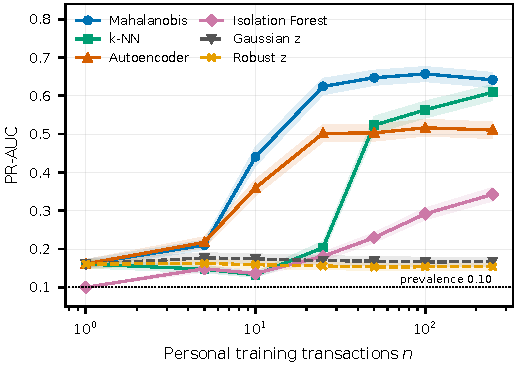
\includegraphics[width=\columnwidth]{figures/fig_berka_curves.pdf}
\caption{Data efficiency on real bank histories (Berka, Protocol~I, 300 accounts). PR-AUC of six personal detectors against the number of personal training transactions $n$; shaded bands are 95\% bootstrap intervals over accounts. Mahalanobis distance and the autoencoder rise steeply and saturate early, $k$-NN rises sharply between $n=25$ and $50$, and the two univariate $z$-scores stay flat at every size.}
\label{fig:berka}
\end{figure}

\begin{table}[!t]
\caption{Mean PR-AUC of personal detectors on Berka (Protocol~I, 300 accounts; prevalence baseline 0.100). Best per row in bold; ties at $n=1$ not marked.}
\label{tab:berka}
\centering\footnotesize\setlength{\tabcolsep}{3.2pt}
\begin{tabular}{r cccccc}
\toprule
$n$ & Mahal. & $k$-NN & Autoenc. & IForest & Gauss.\ z & Robust z \\
\midrule
1   & 0.161 & 0.161 & 0.161 & 0.100 & 0.161 & 0.161 \\
5   & 0.210 & 0.147 & \textbf{0.218} & 0.149 & 0.177 & 0.162 \\
10  & \textbf{0.441} & 0.132 & 0.360 & 0.136 & 0.174 & 0.159 \\
25  & \textbf{0.625} & 0.204 & 0.502 & 0.181 & 0.170 & 0.156 \\
50  & \textbf{0.647} & 0.523 & 0.503 & 0.230 & 0.168 & 0.153 \\
100 & \textbf{0.657} & 0.563 & 0.517 & 0.292 & 0.166 & 0.153 \\
250 & \textbf{0.642} & 0.609 & 0.511 & 0.343 & 0.167 & 0.153 \\
\bottomrule
\end{tabular}
\end{table}

\begin{table}[!t]
\caption{Saturation fits and sufficiency thresholds on Berka. Fits are $y(n)=y_{\max}-(y_{\max}-y_0)e^{-n/\tau}$. Rel-90 and Rel-95 are the relative thresholds of \cref{sec:protocol}; a dash means the criterion is never met on the evaluated grid.}
\label{tab:thresholds}
\centering\footnotesize\setlength{\tabcolsep}{3.5pt}
\begin{tabular}{l ccc ccc}
\toprule
Detector & $y_{\max}$ & $\tau$ & $R^2$ & Rel-90 & Rel-95 & Stability \\
\midrule
Mahalanobis      & 0.658 & 11.5 & 0.970 & 25  & 25  & --- \\
Autoencoder      & 0.518 & 11.1 & 0.980 & 25  & 25  & --- \\
$k$-NN           & 0.633 & 50.9 & 0.912 & 100 & 250 & --- \\
Isolation Forest & 0.350 & 71.2 & 0.985 & 250 & 250 & --- \\
Robust z         & 0.153 & 21.7 & 0.924 & 1   & --- & 25 \\
Gaussian z       & 0.170 & 0.25 & 0.469 & 1   & --- & 50 \\
\bottomrule
\end{tabular}
\end{table}

\Cref{fig:berka,tab:berka} show three regimes. Mahalanobis distance and the autoencoder rise steeply and saturate early. The $k$-NN detector is flat or declining to $n=25$, then rises by 0.320 between 25 and 50 and keeps gaining. Both univariate $z$-scores are flat at every size. For Mahalanobis the marginal gains are $+0.049$ ($1\to5$), $+0.231$ ($5\to10$), $+0.184$ ($10\to25$), $+0.022$ ($25\to50$), $+0.010$ ($50\to100$) and $-0.016$ ($100\to250$): 98\% of the total observed gain arrives by $n=50$, and the last step is negative.

Four of the six curves are well described by a saturating exponential (\cref{tab:thresholds}). The Gaussian-$z$ fit ($R^2=0.469$, nonsensical $y_0=-0.370$) is uninformative because the underlying curve is flat, which is why we report $R^2$ beside the parameters.

\paragraph{Three definitions of sufficiency, three answers}
The relative-90 threshold is 25 for Mahalanobis and the autoencoder, 100 for $k$-NN and 250 for Isolation Forest. It is measured against the best \emph{observed} value, so a curve still rising at $n=250$ yields an optimistic threshold; Isolation Forest is such a curve, while the Mahalanobis curve has stopped rising and its reference is sound. The relative criterion also answers ``when does this detector stop improving'', not ``when is it any good'': the robust-$z$ detector earns a threshold of 1 because it reaches 90\% of its worthless best immediately. The stability criterion is undefined for every detector that works. The across-account standard deviation of PR-AUC never settles at or below its own median for Mahalanobis, $k$-NN, the autoencoder or Isolation Forest at any size; it is defined only for the two flat baselines, which are stably useless. The mean curve therefore hides large individual variation that does not shrink with more data. The thresholds are read off the coarse grid $\{1,5,10,25,50,100,250\}$: ``25'' is the first grid point at which the criterion holds, and the true crossing lies between 10 and 25, where Mahalanobis stands at 67\% of its best at $n=10$ and 95\% at $n=25$.

\paragraph{The threshold is not an artefact of one cohort}
Over five independent cohort draws, the relative-90 threshold for Mahalanobis is exactly 25 at every seed, with best observed PR-AUC between 0.656 and 0.664. The across-seed standard deviation of mean PR-AUC ranges from 0.003 (at $n=50$) to 0.010 (at $n=1$), small against the curve's rise of roughly 0.5.

\subsection{Personal, Population and Hybrid Models}\label{sec:arms}

\begin{figure}[!t]
\centering
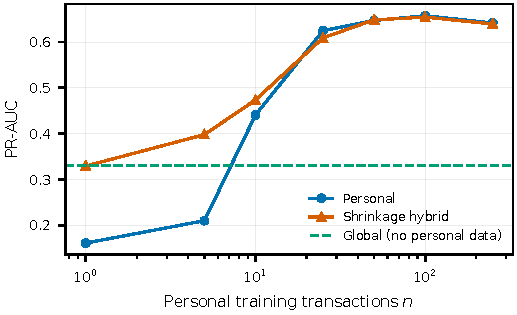
\includegraphics[width=\columnwidth]{figures/fig_arms.pdf}
\caption{Personal, population (global) and shrinkage-hybrid Mahalanobis detectors on Berka. The personal model falls below the global model until $n\approx10$; the hybrid starts at the global level, tracks or exceeds the personal model at every $n$ below 25, and is indistinguishable from it from $n=25$ on.}
\label{fig:arms}
\end{figure}

\begin{table}[!t]
\caption{Mahalanobis on Berka: personal versus global (constant PR-AUC 0.330) and shrinkage hybrid versus personal, paired over 300 accounts. All personal-versus-global Holm $p<0.001$. Final column: hybrid minus personal (Holm $p$).}
\label{tab:arms}
\centering\footnotesize\setlength{\tabcolsep}{2.6pt}
\begin{tabular}{r cc cc}
\toprule
$n$ & Personal & Hybrid & Pers.\ $-$ Global [95\% CI] & Hyb.\ $-$ Pers.\ ($p$) \\
\midrule
1   & 0.161 & 0.329 & $-0.169$ [$-0.196$, $-0.142$] & $+0.168$ ($<$0.001) \\
5   & 0.210 & 0.398 & $-0.120$ [$-0.144$, $-0.096$] & $+0.188$ ($<$0.001) \\
10  & 0.441 & 0.474 & $+0.111$ [$+0.082$, $+0.140$] & $+0.033$ (0.078) \\
25  & 0.625 & 0.609 & $+0.295$ [$+0.265$, $+0.324$] & $-0.016$ (0.795) \\
50  & 0.647 & 0.648 & $+0.317$ [$+0.290$, $+0.345$] & $+0.001$ (1.000) \\
100 & 0.657 & 0.654 & $+0.327$ [$+0.299$, $+0.355$] & $-0.003$ (1.000) \\
250 & 0.642 & 0.639 & $+0.311$ [$+0.284$, $+0.338$] & $-0.002$ (1.000) \\
\bottomrule
\end{tabular}
\end{table}

A population model built from other people's data beats the person's own history below a crossover that depends on the detector. For Mahalanobis the personal model is worse than the global model through $n=5$ (rank-biserial effect $-0.544$) and better from $n=10$ ($+0.465$, \cref{tab:arms}). For $k$-NN, with a global PR-AUC of 0.465, the personal model is worse through $n=25$ ($-0.261$, effect $-0.883$) and better from $n=50$ ($+0.059$, rising to $+0.145$ at 250). At each of the five cohort seeds personal Mahalanobis first exceeds the global model at exactly $n=10$, even though the global model's own mean PR-AUC varies with the donor draw from 0.262 to 0.330. Personalisation is therefore not a safe default in the sparse regime.

The shrinkage hybrid removes the cold-start penalty (\cref{fig:arms,tab:arms}). It improves on the personal model by 0.168 at $n=1$ and 0.188 at $n=5$, and from $n=25$ no difference is detectable (Holm $p\ge0.795$, differences at most 0.016). It is never detectably worse than the personal model and never meaningfully below the global model. The weight $n/(n+\kappa)$ removes the penalty at no measurable cost at large $n$.

\paragraph{Where hybridisation fails}
In the simulation the hybrid plateaus at PR-AUC 0.401 while the personal model reaches 0.924. The simulation's strongest features are personal novelty indicators (is this merchant one \emph{you} have used), computed against a reference history; the hybrid computes them against the population reference, which destroys the signal that matters. Parameter shrinkage cannot recover information the feature representation has already discarded. Shrinkage hybrids therefore reduce the personal data requirement when the personal signal lives in the \emph{parameters} of a shared representation, as in the Berka features, and fail when it lives in the representation itself, as in the simulation's.

\subsection{The Operating Point Depends on the Calibration Rule}\label{sec:calibration}

PR-AUC measures ranking; a deployed detector also needs an alert threshold. \Cref{tab:calib} compares the two calibration rules of \cref{sec:protocol} for personal Mahalanobis on the primary cohort.

\begin{table}[!t]
\caption{Personal Mahalanobis on Berka under in-sample and leave-one-out (LOO) calibration (nominal FPR 0.05; 300 accounts). At $n=1$ the in-sample rule flags 99.9\% of transactions and the LOO rule is undefined.}
\label{tab:calib}
\centering\footnotesize\setlength{\tabcolsep}{2.8pt}
\begin{tabular}{r cc cccc}
\toprule
& \multicolumn{2}{c}{In-sample} & \multicolumn{4}{c}{LOO} \\
\cmidrule(lr){2-3}\cmidrule(lr){4-7}
$n$ & Flag rate & FPR & Flag rate & FPR & Recall & Precision \\
\midrule
5   & 0.989 & 0.988 & 0.152 & 0.151 & 0.163 & 0.110 \\
10  & 0.960 & 0.956 & 0.012 & 0.007 & 0.058 & 0.667 \\
25  & 0.391 & 0.335 & 0.110 & 0.066 & 0.503 & 0.577 \\
50  & 0.251 & 0.189 & 0.126 & 0.073 & 0.612 & 0.558 \\
100 & 0.196 & 0.134 & 0.134 & 0.076 & 0.658 & 0.533 \\
250 & 0.162 & 0.104 & 0.136 & 0.080 & 0.647 & 0.516 \\
\bottomrule
\end{tabular}
\end{table}

\paragraph{In-sample calibration flags almost everything at small $n$}
At $n=10$ the PR-AUC is 0.441, more than four times the prevalence baseline, yet the in-sample rule flags 96\% of all transactions. The cause is a bias in the rule, not data scarcity. In-sample scores are biased low by construction whenever a model scores the points it was fitted to: a personal Mahalanobis fit on $n\le d=21$ points has a singular covariance, so every training point lies in the span of the fit and scores near zero, and a $k$-NN training point counts itself as a neighbour at distance 0. The 95th percentile of such scores is systematically too low, and more data removes that bias only slowly.

\paragraph{LOO calibration makes the detector silent at $n=10$ and near-nominal from $n=25$}
Under LOO calibration, which is out-of-sample, the same detector flags 1.2\% of transactions at $n=10$ with recall 0.058: ten LOO scores give a threshold dominated by the single most extreme of them. From $n=25$ the FPR is 0.066 against a nominal 0.05, rising slowly to 0.080 at $n=250$, with recall between 0.50 and 0.65. The paired in-sample-minus-LOO difference in FPR is significant at every size (Wilcoxon $p<10^{-36}$), with mean differences of 0.949 at $n=10$, 0.268 at 25 and 0.116 at 50. The PR-AUC at $n=10$ still does not translate into a usable operating point: the detector is silent, not noisy, for as long as its threshold must come from the person's own ten points. The nominal 5\% is missed by 1.6 to 3 points at every size from 25; training points and evaluation-window points are not exchangeable, since the window is later in time, and we did not diagnose the cause, so ``near-nominal'' is not ``well calibrated''.

\begin{table*}[!t]
\caption{Mean FPR under LOO calibration, with the in-sample value in parentheses (nominal 0.05). Six personal detectors and the shrinkage-hybrid Mahalanobis on Berka, 300 accounts at each of five cohort seeds (1{,}500 account-seed rows per cell). Recall under LOO calibration is in \cref{tab:recall}.}
\label{tab:fpr_all}
\centering\footnotesize\setlength{\tabcolsep}{5pt}
\begin{tabular}{l cccccc}
\toprule
Detector & $n=5$ & $n=10$ & $n=25$ & $n=50$ & $n=100$ & $n=250$ \\
\midrule
Gaussian z       & 0.049 (0.263) & 0.012 (0.108) & 0.005 (0.017) & 0.006 (0.007) & 0.007 (0.007) & 0.006 (0.007) \\
Robust z         & 0.045 (0.237) & 0.048 (0.104) & 0.017 (0.016) & 0.013 (0.006) & 0.012 (0.006) & 0.009 (0.006) \\
Mahalanobis      & 0.154 (0.989) & 0.012 (0.958) & 0.066 (0.331) & 0.068 (0.185) & 0.073 (0.132) & 0.083 (0.107) \\
$k$-NN           & 0.492 (0.492) & 0.132 (0.194) & 0.041 (0.098) & 0.054 (0.104) & 0.071 (0.105) & 0.082 (0.111) \\
Isolation Forest & 0.535 (0.236) & 0.205 (0.199) & 0.009 (0.143) & 0.025 (0.113) & 0.042 (0.090) & 0.055 (0.075) \\
Autoencoder      & 0.191 (0.984) & 0.021 (0.667) & 0.049 (0.205) & 0.060 (0.127) & 0.068 (0.100) & 0.077 (0.091) \\
Hybrid           & 0.097 (0.395) & 0.028 (0.266) & 0.040 (0.184) & 0.060 (0.138) & 0.070 (0.114) & 0.080 (0.102) \\
\bottomrule
\end{tabular}
\end{table*}

\paragraph{The effect holds across detectors and cohorts, and its direction varies}
Repeating the comparison for all six personal detectors and the hybrid at the five seeds (\cref{tab:fpr_all}) shows the following.
\begin{itemize}
\item \emph{The Mahalanobis correction is stable across cohorts.} Pooled over five seeds, FPR is 0.012 at $n=10$ and 0.066 at $n=25$, and the across-seed standard deviation of the per-seed mean FPR is at most 0.008 at any size from 5.
\item \emph{The artefact is not specific to Mahalanobis.} The autoencoder's in-sample flag rate at $n=10$ is 0.691 against 0.025 under LOO; the hybrid's is 0.296 against 0.051. In-sample and LOO FPR differ significantly (paired Wilcoxon $p<10^{-4}$) in 39 of 42 detector-by-size cells; the in-sample FPR is higher in 35 and lower in 4 (Isolation Forest at $n=5$; robust $z$ at $n=50$, 100 and 250). The three cells without a detectable difference are Isolation Forest at $n=10$, robust $z$ at $n=25$, and $k$-NN at $n=5$, where the two rules are identical by construction: with $k=n=5$ the in-sample fifth-nearest-neighbour distance, counting the point itself at distance 0, equals the maximum distance to the other four points, which is the LOO score.
\item \emph{A usable operating point near $n=25$ holds only for detectors that also rank well.} At $n=25$ the FPRs of Mahalanobis (0.066), the autoencoder (0.049) and the hybrid (0.040) lie within about 1.6 points of 0.05, with recall 0.37 to 0.50. The $k$-NN detector has FPR 0.041 but recall 0.038 at $n=25$ and stays silent until about $n=50$ (recall 0.386). Isolation Forest has FPR 0.009 and recall 0.018 at $n=25$ and reaches recall of only 0.236 at $n=250$, so no usable operating point appears within the sizes tested, consistent with its PR-AUC curve. The two $z$-score detectors are conservative under LOO and keep recall between 0.035 and 0.055 at every $n\ge25$.
\item \emph{The in-sample rule is not an upper bound on false-positive burden.} Isolation Forest flags more under LOO than in-sample at $n=5$ (flag rate 0.533 against 0.232), the two rules are indistinguishable at $n=10$ (paired $p=0.7$), and robust $z$ has a slightly lower in-sample FPR at $n\ge50$ (by 0.003 to 0.007). The LOO forest is fitted on $n-1$ points and an isolation forest's score normalisation depends on its subsample size, so its LOO scores and the scores of the $n$-point forest are not on exactly the same scale; whether this explains Isolation Forest at $n\le10$ is untested, and that behaviour is not evidence about the detector.
\item \emph{The hybrid has the best small-$n$ operating behaviour.} At $n=10$ its LOO FPR is 0.028 and recall 0.254, against 0.012 and 0.055 for personal Mahalanobis; at $n=5$ the figures are 0.097 and 0.272 against 0.154 and 0.168. This extends the ranking result of \cref{sec:arms} to the operating point; it is an observation from one calibration rule and one anomaly protocol, not a pre-specified significance test.
\end{itemize}

\paragraph{Consequence for the sufficiency threshold}
The measured requirement depends on how the threshold is calibrated as well as on the criterion. Under in-sample calibration the Mahalanobis FPR is still 0.189 at $n=50$ and 0.104 at $n=250$; under LOO calibration it lies within about 3 points of nominal from $n=25$ for Mahalanobis, the autoencoder and the hybrid, but only from about $n=50$ for $k$-NN and not within 250 for Isolation Forest. Any single-number ``$N$ transactions is enough'' claim conceals both the criterion and the calibration rule. The relative-90 ranking thresholds of \cref{tab:thresholds} depend on no threshold rule. Operating-point results for the global arm, Protocol~P, the temporal experiments, the simulation, TabFormer and the audit of \cref{sec:audit} at $n=10$ and 50 use the in-sample rule; because that rule is not an upper bound, they are not worst-case figures either.

\subsection{Recency, Volume and Drift}\label{sec:recency}

Does more history help because of the count of transactions or the span of time they cover? We hold the count at $n=50$ and widen coverage by stride-sampling the history. Inter-arrival gaps are computed against each transaction's true position in the unthinned timeline, so thinning does not change the gap feature's meaning.

\begin{table}[!t]
\caption{Fixed count $n=50$, widening temporal coverage (Berka, 300 accounts). Stride~1 is the 50 most recent transactions; $\Delta$ is the paired PR-AUC difference from stride~1.}
\label{tab:stride}
\centering\footnotesize\setlength{\tabcolsep}{4pt}
\begin{tabular}{l c cc cc}
\toprule
 & Median & \multicolumn{2}{c}{Mahalanobis} & \multicolumn{2}{c}{$k$-NN} \\
\cmidrule(lr){3-4}\cmidrule(lr){5-6}
Arm & span (days) & PR-AUC & $\Delta$ & PR-AUC & $\Delta$ \\
\midrule
Stride 1 & 224 & 0.663 & --- & 0.540 & --- \\
Stride 2 & 457 & 0.660 & $-0.004$ & 0.478 & $-0.062$ \\
Stride 4 & 946 & 0.627 & $-0.036$ & 0.430 & $-0.110$ \\
\bottomrule
\end{tabular}
\end{table}

\Cref{tab:stride} shows that for Mahalanobis stride 2 changes PR-AUC by $-0.004$ (not detectable, $p=0.304$) and stride 4 by $-0.036$ ($p<0.001$, effect $-0.300$); for $k$-NN both strides lose significantly ($p<0.001$). Coverage and sampling density cannot be varied independently at fixed count: a control arm that keeps the 50 transactions recent but thins them by four necessarily reaches back four times further, and it did (span 950 against 946 days, near-identical results). The effect of span is therefore not separable from the effect of density in this design. Together with \cref{sec:curves} the evidence is clear on one point: raising the count from 50 to 250 at natural density changes Mahalanobis PR-AUC from 0.647 to 0.642, while drawing the same 50 transactions from a span four times longer costs 0.036. Within Berka, neither more transactions nor more time helps once about 50 recent transactions are available, and reaching further back is mildly harmful: recency dominates volume.

\paragraph{Drift does not explain the cost of older history}
Behavioural drift is the natural explanation, so we test it directly. For each account, drift is the Mahalanobis distance between the 150 transactions added when history grows from 100 to 250 and the 100 transactions already present at $n=100$, measured in the account's own recent coordinate system: both blocks are mapped to the detectors' causal features, standardised by a scaler fitted on the recent block only, and compared through the recent block's ridge-regularised covariance. This is ``how many of my own recent standard deviations away is my older behaviour'', computed independently of any detector score or anomaly label. Drift is substantial and accumulates with lag: its median is 0.69 and mean 1.00 (maximum 12.6), and a lag sweep shows mean drift rising from 0 at lag 0 to 1.72 at lag 25 and plateauing near 3.2 to 3.6 by 150 to 200 transactions back. Older behaviour does look different from recent behaviour. But an account's drift magnitude does not predict that account's own marginal PR-AUC gain from 100 to 250 transactions: Spearman $\rho=-0.081$ for Mahalanobis and $+0.070$ for $k$-NN (both Holm $p=0.32$, $n=300$). Drift accumulates with lag, yet it does not explain which accounts lose performance when older history is added. The mechanism behind the negative $100\to250$ step, and behind the cost of reaching further back, remains open.

\subsection{Robustness to the Anomaly Definition}\label{sec:robust}

Under Protocol~P (amount multiplied by 5), the ordering of detectors changes. The Gaussian-$z$ detector, flat under Protocol~I (0.166 at $n=100$), becomes competitive (0.294), as expected for a perturbation applied to amount alone. Mahalanobis remains best but at a lower level (0.455 at $n=100$, against 0.657), with PR-AUC 0.258, 0.423 and 0.453 at $n=1$, 25 and 250; $k$-NN reaches 0.153, 0.212 and 0.217 and Isolation Forest 0.163, 0.194 and 0.211 at $n=25$, 100 and 250. The Mahalanobis relative-90 threshold is again 25. The threshold of roughly 25 transactions therefore holds across two structurally different anomaly definitions, while the \emph{level} of achievable PR-AUC is strongly protocol-dependent and does not transfer between them.

\subsection{Behavioural Variability and the Requirement}\label{sec:variability}

\begin{figure}[!t]
\centering
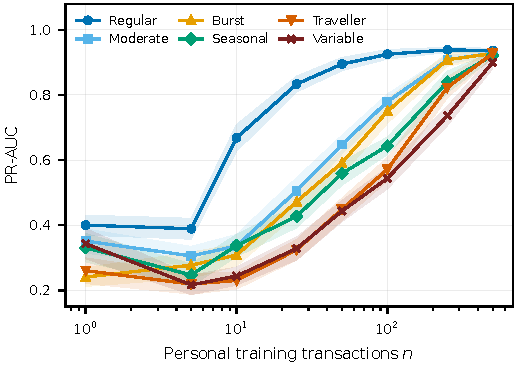
\includegraphics[width=\columnwidth]{figures/fig_sim_archetypes.pdf}
\caption{Simulation: personal Mahalanobis PR-AUC by behavioural archetype (mean $\pm$ 1.96 standard errors over 40 individuals per archetype). The regular archetype saturates by $n\approx50$; traveller and variable individuals need several hundred transactions, yet all archetypes converge to similar ceilings.}
\label{fig:sim}
\end{figure}

\begin{table}[!t]
\caption{Simulation: relative-90 threshold and best PR-AUC of personal Mahalanobis by archetype.}
\label{tab:archetypes}
\centering\footnotesize\setlength{\tabcolsep}{6pt}
\begin{tabular}{l cc}
\toprule
Archetype & Rel-90 threshold & Best PR-AUC \\
\midrule
Regular   & 50  & 0.939 \\
Moderate  & 250 & 0.929 \\
Seasonal  & 250 & 0.923 \\
Burst     & 250 & 0.927 \\
Traveller & 500 & 0.928 \\
Variable  & 500 & 0.900 \\
\bottomrule
\end{tabular}
\end{table}

\paragraph{Under controlled manipulation, variability predicts the requirement}
With variability set by the generative parameters, every descriptor predicts each individual's relative-90 threshold (all Holm $p<0.001$): number of distinct merchants ($\rho=+0.708$), category entropy ($+0.700$), merchant entropy ($+0.700$), log-amount standard deviation ($+0.673$), location entropy ($+0.617$) and inter-arrival coefficient of variation ($+0.484$). The archetypes differ tenfold in requirement, from 50 to 500 transactions (\cref{fig:sim,tab:archetypes}), while converging to similar ceilings (best PR-AUC 0.900 to 0.939): variability changes the \emph{rate} of learning far more than its ceiling.

\paragraph{In real accounts, no descriptor predicts the requirement}
We computed eight descriptors on each Berka account's 250-transaction history (amount coefficient of variation, robust amount coefficient of variation, log-amount interquartile range, operation entropy, \texttt{k\_symbol} entropy, operation diversity, inter-arrival coefficient of variation and credit share) and correlated each with the account's own relative-90 threshold. After Holm correction over the eight, all $p\ge0.867$ and all $|\rho|\le0.12$. The test uses the 183 accounts with a defined threshold; the other 117 (39\%) never reached and held 90\% of their own best value, so the 183 are a non-random subset of better-behaved accounts. At that size a two-sided Spearman test reaches about 80\% power only for $|\rho|\gtrsim0.21$ before correction, so the null excludes moderate-to-strong effects and leaves weak ones open. Diverse operation and \texttt{k\_symbol} usage does correlate with higher \emph{best achievable} PR-AUC (uncorrected $\rho=+0.167$ to $+0.209$, $p=0.005$ to 0.024), plausibly because a distinctive profile is easier to separate from an impostor's.

\paragraph{Three explanations remain}
The Berka descriptors may be too thin: the dataset has no merchant, category or location channels, which are exactly the channels carrying the simulation's effect. The real cohort's variability range may be too narrow, since all accounts are ordinary retail accounts at one bank. Or observed variability may be confounded with account type, tenure and product mix in ways the simulation excludes by construction. The simulation shows that the effect exists when the generative parameters are what theory says they are; it is not evidence that the effect exists in real data. A partial test uses TabFormer, whose schema has the missing channels: there, state entropy does predict an entity's relative-90 threshold after Holm correction ($\rho=+0.19$, $p=0.028$; merchant diversity is marginal at $p=0.148$), unlike every descriptor on Berka. This is consistent with channel availability being what the Berka null lacked; because TabFormer is synthetic, it cannot turn the real-data null into a positive finding.

\paragraph{Anomaly classes differ in their data requirements}
In the simulation, the mean score percentile of Mahalanobis (1.0 is most anomalous) shows that categorical-novelty anomalies start near chance and improve steeply, since recognising an unfamiliar merchant requires having seen the familiar ones: merchant, category and geographic anomalies rise from 0.545, 0.547 and 0.642 at $n=1$ to 0.947, 0.957 and 0.969 at $n=250$. Amount and temporal anomalies start above chance (0.789 and 0.721) and improve least (0.861 and 0.845 at $n=250$), because one observation already locates a distribution's centre roughly. Multivariate anomalies are effectively saturated by $n=50$ (0.999). Amount detectability falls from 0.789 at $n=1$ to 0.576 at $n=10$ before recovering; the apparent competence at $n=1$ is an artefact of degenerate variance, not detection.

\subsection{Replication on a Second Dataset}\label{sec:tabformer}

\begin{figure}[!t]
\centering
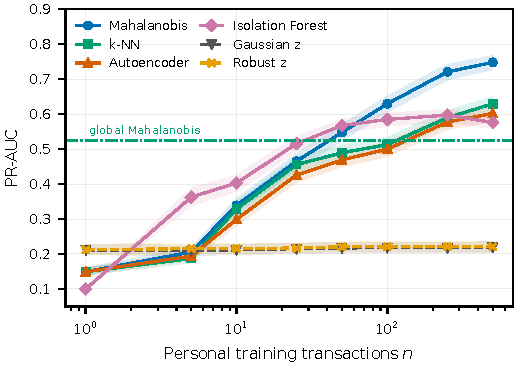
\includegraphics[width=\columnwidth]{figures/fig_tabformer_curves.pdf}
\caption{Data efficiency on TabFormer (\emph{synthetic} card data; Protocol~I; 300 entities; bands are 95\% bootstrap intervals). The steep-rise, early-plateau shape and the flat $z$-scores recur, but Isolation Forest is the best detector at $n=5$ to $50$, the opposite of its position on Berka.}
\label{fig:tabformer}
\end{figure}

Every number in this subsection comes from TabFormer, a synthetic dataset, and none is pooled with the real-data results. The question is whether the shape found on Berka (steep early rise, plateau, a global-personal crossover, an early and stable threshold) is specific to one dataset.

\paragraph{The shape replicates, with a later threshold}
Mahalanobis again rises steeply and attains the highest ceiling (0.748 at $n=500$), and both $z$-scores are flat at 0.21 to 0.22 at every size (\cref{fig:tabformer}). The Mahalanobis relative-90 threshold is 250, against Berka's 25. Two candidate reasons, both untested, are that TabFormer's 26-dimensional feature space needs more observations before an $n\le d$ covariance estimate stops being singular, and that the global model here is much stronger (PR-AUC 0.524 against Berka's 0.330), which raises the bar that the personal curve must clear to look saturated.

\paragraph{The global-personal crossover moves with the strength of the global model}
Personal Mahalanobis minus global is $-0.375$ at $n=1$, $-0.059$ at 25 (Holm $p<0.001$), $+0.023$ at 50 ($p=0.094$), $+0.105$ at 100 and $+0.223$ at 500 (both $p<0.001$). The crossover falls between $n=25$ and $100$, later than Berka's 5 to 10, as expected if a stronger population baseline raises the bar that personalisation must clear. Personalisation is harmful below a detector- and dataset-dependent crossover on both datasets.

\paragraph{Detector ranking under scarcity reverses}
On Berka, Isolation Forest is the worst detector at every history size, from PR-AUC 0.100 at $n=1$ (exactly the prevalence baseline) to 0.343 at 250, and its fitting is the most expensive: at $n=250$ the median fit time is 0.46\,ms for Mahalanobis, 5.0\,ms for $k$-NN, 22.9\,ms for the autoencoder and 156.3\,ms for Isolation Forest. On TabFormer it is the single best detector at $n=5$, 10, 25 and 50 (0.362 against Mahalanobis's 0.206 at $n=5$, and 0.567 against 0.548 at $n=50$) and falls behind Mahalanobis only from $n=100$ (0.585 against 0.630). A candidate explanation, untested, is that TabFormer's higher-dimensional, one-hot-heavy space gives isolation splits more structure to exploit at small samples. The answer to whether sophisticated detectors beat simple statistics under scarcity is therefore dataset-dependent: on Berka the best detector is a shrinkage-regularised covariance estimate, and on TabFormer the answer differs at small $n$.

\paragraph{Fraud labels could not be evaluated}
An exploratory protocol against the generator's own fraud label found no positive example: none of the 300 evaluated entities' 60-transaction windows contained a generator-labelled fraud, consistent with the 0.122\% corpus-wide prevalence (about 0.07 expected per window).

\subsection{Disparate-Impact Audit}\label{sec:audit}

Sparse-history users are the people the study is most about, so we test whether false-positive burden concentrates by district economics. We join the 300 evaluated accounts to their district's average salary, unemployment rate, urbanisation ratio and region, and test whether the personal Mahalanobis detector's FPR varies with them (Kruskal-Wallis across 8 regions; Spearman with Holm correction over the three continuous variables). The audit is ecological: Berka carries no per-person demographic field.

\begin{table}[!t]
\caption{Disparate-impact audit under LOO calibration (Berka, 300 accounts). Spearman $\rho$ between an account's FPR and its district's attribute (Holm $p$), and Kruskal-Wallis $p$ across regions. Mean FPR is 0.066, 0.073 and 0.076.}
\label{tab:audit}
\centering\footnotesize\setlength{\tabcolsep}{3pt}
\begin{tabular}{r ccc c}
\toprule
$n$ & Avg.\ salary & Unemployment & Urban ratio & Region \\
\midrule
25  & $-0.115$ (0.137) & $+0.012$ (0.838) & $-0.110$ (0.137) & 0.70 \\
50  & $-0.053$ (0.719) & $-0.026$ (0.719) & $-0.077$ (0.554) & 0.53 \\
100 & $-0.130$ (0.073) & $+0.104$ (0.145) & $-0.073$ (0.211) & 0.49 \\
\bottomrule
\end{tabular}
\end{table}

No relationship is Holm-significant (\cref{tab:audit}). Under the in-sample rule at $n=10$ and 50 all $|\rho|\le0.07$ and no Holm $p$ falls below 0.75; the $n=10$ half carries almost no information, because the in-sample FPR sits near its ceiling of 0.96 for every account. The salary correlation is negative at all three LOO sizes (higher-salary districts have somewhat lower FPR), with uncorrected $p=0.046$ at $n=25$ and 0.024 at $n=100$; with $|\rho|\le0.13$, at or below what 300 accounts can reliably detect (about 80\% power for $|\rho|\gtrsim0.16$), it is reported here as a trend, not an effect. False-positive burden is not visibly concentrated by district-level economic disadvantage in this dataset; whether it concentrates by age, tenure, immigration status or other axes that Berka cannot supply remains untested.

\section{Discussion}\label{sec:discussion}

\paragraph{What the evidence establishes}
On real transaction histories, personalised behavioural anomaly detection improves steeply between 5 and 25 personal transactions and is essentially saturated by 50. The relative-90 threshold of 25 is identical across five cohort draws and across two anomaly definitions, so it reflects the estimation problem rather than one cohort or one protocol. Ranking quality and operating behaviour reach adequacy at about the same history size once the alert threshold is calibrated out-of-sample (LOO FPR 0.066 at $n=25$ against a nominal 0.05); what separates them is a narrower point, that at $n=10$ a PR-AUC of 0.441 yields no usable operating point under either calibration rule (in-sample flags 96\%, LOO flags 1.2\%). Personalisation is worse than a population model below a detector- and dataset-dependent crossover, and a history-weighted shrinkage hybrid removes that penalty when the personal signal lives in the parameters of a shared representation. Detector rankings under scarcity are dataset-dependent. Variability governs the \emph{rate} of learning under controlled manipulation, though not detectably in real Berka accounts. Recent history suffices, and a district-level audit finds no Holm-significant concentration of false positives.

\paragraph{What remains interpretation}
That the real-data null on variability reflects thin descriptors rather than a genuinely absent effect is an interpretation. The TabFormer result (a Holm-significant state-entropy effect on a dataset with a geographic channel) makes it more credible than the alternative that retail banking has no such effect, without resolving it, since TabFormer is synthetic. The mechanism behind the negative $100\to250$ marginal gain and the cost of reaching further back is open: drift is real and lag-dependent but does not predict which accounts lose.

\paragraph{Practical implication}
For the best real-data detector, the answer to ``how much history is enough'' is about 25 transactions for ranking quality, about 25 before the FPR is near nominal under LOO calibration, and no number that guarantees any individual is well served. The third clause matters most. The across-account spread of PR-AUC never stabilised at any size we evaluated, so a system that meets a target on average still fails badly for a substantial minority of users; a population average is the wrong unit for a decision applied per person. A system should therefore use a hybrid that degrades to population behaviour when personal history is thin, hold recent history rather than all history, treat a detector that ranks well as not yet a detector that can be deployed, and verify on its own data any claim about which detector is best under scarcity.

\section{Limitations}\label{sec:limits}

\paragraph{Data}
The real evidence is one dataset from one bank in one country, 1993 to 1998 retail banking, with day-resolution timestamps and no merchant, category or geographic fields. The three simulated anomaly classes with the steepest data requirements (merchant, category, geographic) therefore could not be tested on real behaviour. TabFormer adds those channels, but it is synthetic, so generalisation to modern real card payments is untested; the reversal of Isolation Forest's ranking between the two datasets shows that this limit matters in practice. Real history sizes stop at 250 because of dataset depth, and several TabFormer curves are still rising at 250, which hints at, but is not evidence for, what a deeper real dataset would show. The evaluated cohort (at least 310 transactions) is the more active half of the accounts and is not representative of the sparse-history users this study is most about.

\paragraph{Protocol}
Neither injection protocol produces fraud, and neither models an adversary who imitates the account holder; such an adversary would choose transactions near the victim's behavioural centre, the hardest case and the one we cannot evaluate. Protocol~I makes timing non-discriminative by construction. The 10\% injection rate is far above realistic fraud prevalence, so absolute PR-AUC values do not transfer to a realistic base rate; the shape of the curves is the transferable quantity. Transaction count and temporal coverage cannot be separated at fixed count.

\paragraph{Modelling and calibration}
The hybrid strength $\kappa=25$ was fixed in advance; tuning it would likely improve the hybrid but would invalidate the comparison on our data. The autoencoder is deliberately small. Thresholds are read from mean curves on a coarse grid, the per-account threshold distribution is heavy-tailed with 39\% undefined, and the fitted $\tau$ values are not cross-validated against alternative model forms such as a power law. LOO calibration is one of several out-of-sample rules; split-half and population-derived thresholds were not tried, and for Isolation Forest at $n\le10$ the scale mismatch of its LOO forest is an untested confound. LOO operating-point results cover Berka under Protocol~I; the other operating-point figures (\cref{sec:calibration}) use the in-sample rule.

\paragraph{Statistics}
Cohort selection was repeated at five seeds for the Berka Protocol~I curves and the simulation's Mahalanobis and $k$-NN curves. Protocol~P, the simulation's Isolation Forest and autoencoder, the stride experiment, TabFormer, the drift measurement and the audit each rest on one realised sample. TabFormer was verified from a single download source. With 300 paired entities, Wilcoxon $p$ values are extremely small even for effects of no practical size, which is why effect sizes accompany them; the hybrid's $-0.033$ difference at $n=10$ is one such case.

\section{Ethical Considerations}\label{sec:ethics}

\paragraph{Deviation is not suspicion}
The transactions our detectors flag are, by construction, transactions that differ from a person's past. In life those are holidays, house moves, medical costs, a new job, a death in the family, leaving an abusive relationship. A system that escalates deviation to suspicion penalises people for changing.

\paragraph{False positives are not symmetric with false negatives}
A missed anomaly costs an institution money; a false positive can mean a declined card abroad, a frozen account during an emergency, or an account holder treated as a suspect. Our best real-data detector at $n=50$ has an FPR of 7.3\% under LOO calibration (18.9\% under in-sample calibration) against a nominal 5\%, and at realistic transaction volumes even 7\% means very many wrongly flagged legitimate transactions.

\paragraph{Sparse-history users}
The people with the least history are new customers, young people, recent immigrants and people re-entering the formal banking system. For them a personal model either floods them with alerts (in-sample calibration) or says nothing (LOO calibration at $n=10$), and below the crossover a population or hybrid model outperforms it. Deploying personalisation without a history floor serves exactly these users worst.

\paragraph{Discrimination}
Behavioural features are proxies for life circumstances: irregular income, cash reliance and geographic mobility correlate with class, occupation, immigration status and disability, and a detector calibrated on regular salaried behaviour treats irregular lives as anomalous by default. Our district-level audit (\cref{sec:audit}) finds no Holm-significant relationship between FPR and average salary, unemployment, urbanisation or region, but with 300 accounts it cannot exclude weak effects, and Berka carries no per-person demographic field, so age, tenure, immigration status and disability are untested. The audit narrows the concern; it does not clear it, and no system of this kind should be deployed without an individual-level audit on the axes we could not test.

\paragraph{Privacy, explainability and data handling}
Personal transaction histories are among the most revealing data about a person, and per-user modelling requires retaining and processing them continuously. That recent history suffices and older history is mildly harmful (\cref{sec:recency}) is a rare case where a privacy interest and a performance interest align: shorter retention appears to cost nothing here. A Mahalanobis distance is a scalar with no account of which behaviour was unusual; any deployment that affects a person's access to their money should state the reason and support contest and correction. The Berka data were anonymised by their publisher; we redistribute no raw records, work only at account-identifier level and make no attempt at re-identification.

\paragraph{Appropriate use}
The thresholds reported here describe when a personal baseline ranks well on these data. They are not a licence to deploy a detector at $N$ transactions, and a flagged transaction is not grounds for adverse action against a customer.

\section{Conclusion}\label{sec:conclusion}

We measured how much of a person's own transaction history an unsupervised behavioural anomaly detector needs, on real bank histories, in a controlled simulation and on a structurally different synthetic card dataset, using a ground-truth protocol defined by provenance rather than by any statistical rule. A sufficiency point exists and arrives earlier than the framing of the question suggests: about 25 personal transactions for ranking quality with the best real-data detector, saturation by 50, and the same shape, with a later threshold, on card-structured data whose global baseline is much stronger. Below that point a population model built from other people's behaviour does better than the person's own history, and a shrinkage hybrid that degrades to the population when history is thin removes the penalty at no measurable cost later.

The single number is the least useful part of the answer. Whether a ranking-quality threshold translates into a usable alert threshold depends on how the alert threshold is calibrated: scoring a model's own training data makes it flag 96\% of transactions at 10 personal transactions, and leave-one-out calibration makes the same model nearly silent there and near-nominal from 25. Detector rankings under scarcity are dataset-dependent, behavioural variability changes the requirement tenfold when manipulated but is not detectable across real accounts, and a direct drift measurement does not explain why older history hurts. No history size made performance stable across individuals, which undermines any per-person guarantee derived from a population average.

Two extensions would sharpen these results. A finer history grid between 10 and 25, together with alternative out-of-sample threshold rules (split-half and population-derived) on both datasets, would localise the sufficiency point and test whether LOO calibration is the right rule. A targeted evaluation on entities with historical generator-labelled fraud, and a deeper real dataset carrying merchant fields and individual-level demographics, would test the findings against fraud labels and enable an individual-level fairness audit.


\appendices
\section{Leave-One-Out Recall by Detector}\label{app:recall}

\Cref{tab:recall} gives the recall that accompanies the LOO false-positive rates of \cref{tab:fpr_all}, with the same cohorts and seeds.

\begin{table}[!t]
\caption{Mean recall under LOO calibration on Berka (300 accounts, five seeds).}
\label{tab:recall}
\centering\footnotesize\setlength{\tabcolsep}{3pt}
\begin{tabular}{l cccccc}
\toprule
Detector & $n=5$ & 10 & 25 & 50 & 100 & 250 \\
\midrule
Gaussian z       & 0.070 & 0.038 & 0.047 & 0.053 & 0.054 & 0.055 \\
Robust z         & 0.057 & 0.063 & 0.037 & 0.035 & 0.037 & 0.035 \\
Mahalanobis      & 0.168 & 0.055 & 0.499 & 0.596 & 0.642 & 0.640 \\
$k$-NN           & 0.455 & 0.093 & 0.038 & 0.386 & 0.545 & 0.602 \\
Isolation Forest & 0.519 & 0.167 & 0.018 & 0.076 & 0.164 & 0.236 \\
Autoencoder      & 0.226 & 0.064 & 0.366 & 0.445 & 0.480 & 0.483 \\
Hybrid           & 0.272 & 0.254 & 0.468 & 0.586 & 0.633 & 0.635 \\
\bottomrule
\end{tabular}
\end{table}

\section{Reproducibility}\label{app:repro}

\paragraph{Environment}
Python 3.14.6 in a fresh virtual environment with pandas 3.0.6, NumPy 2.5.3, scikit-learn 1.9.1, SciPy 1.18.1 and Matplotlib 3.11.2, resolved by \texttt{pip} against the repository's \texttt{requirements.txt}. No GPU is used and the autoencoder is implemented in NumPy. Wall-clock times depend on hardware and load and are recorded in run logs, not stated here.

\paragraph{Data integrity}
The Berka loader checks all eight tables against the record counts published by the dataset's authors and raises on mismatch; the content of every table was also cross-checked byte-for-byte, after line-ending normalisation, against a second independent mirror (digests in \texttt{docs/data\_integrity\_report.json}). TabFormer's 24{,}386{,}900 transactions and 2{,}000 users were counted independently by a full chunked pass over the downloaded file; it has single-source provenance.

\paragraph{Parameters}
\Cref{tab:params} lists the fixed experimental parameters. The master seed is 20260920 throughout; the five-seed replication sweeps 20260920 to 20260924 by design. Per-entity seeds are derived as $\text{seed}\times100003+\text{account id}$ for Berka and from a stable hash of the entity string for TabFormer.

\begin{table}[!t]
\caption{Experimental parameters.}
\label{tab:params}
\centering\footnotesize\setlength{\tabcolsep}{4pt}
\begin{tabular}{p{0.38\columnwidth} p{0.55\columnwidth}}
\toprule
Parameter & Value \\
\midrule
Evaluation window & 60 transactions (Berka, TabFormer); 100 (simulation) \\
Injection rate & 0.10 \\
History sizes & $\{1,5,10,25,50,100,250\}$ Berka; plus 500 for simulation and TabFormer \\
Evaluated / donor entities & 300 / 400 (Berka, TabFormer) \\
Eligibility & Berka $\ge310$ transactions (1{,}319 qualify); TabFormer $\ge560$ (4{,}538 of 6{,}139 pairs) \\
Nominal FPR $\alpha$ & 0.05 \\
Hybrid $\kappa$ & 25 \\
Bootstrap resamples & 2{,}000 \\
Isolation Forest & 200 trees, $\texttt{max\_samples}=\min(256,n)$ \\
Autoencoder & $d$-4-$d$, tanh, 300 epochs, Adam (learning rate 0.01), weight decay $10^{-4}$ \\
$k$-NN & $k=5$ \\
Drift blocks & recent 100 transactions; older 150 (positions 101 to 250 back) \\
Audit history sizes & $n=10,50$ (in-sample); $n=25,50,100$ (LOO) \\
\bottomrule
\end{tabular}
\end{table}

\paragraph{Reproduction}
All commands run from the repository root as \texttt{python -m experiments.<module>} after \texttt{pip install -r requirements.txt} and \texttt{python -m src.data\_loader}. \Cref{tab:modules} maps results to modules; figures for this paper are regenerated by \texttt{paper/make\_figures.py} from the result tables.

\begin{table}[!t]
\caption{Result-to-module map (modules under \texttt{experiments/}).}
\label{tab:modules}
\centering\footnotesize\setlength{\tabcolsep}{4pt}
\begin{tabular}{p{0.46\columnwidth} p{0.47\columnwidth}}
\toprule
Result & Module \\
\midrule
Pipeline validation & \texttt{pilot} \\
Berka curves, arms, Protocol~P & \texttt{run\_all}, \texttt{analyse} \\
Stride experiment & \texttt{e3\_temporal\_fixed} \\
Simulation & \texttt{run\_simulation}, \texttt{analyse\_simulation} \\
Five-seed replication & \texttt{e5\_multiseed} \\
Drift measurement & \texttt{e6\_drift} \\
TabFormer & \texttt{run\_tabformer}, \texttt{analyse\_tabformer} \\
Disparate-impact audit & \texttt{e8\_disparate\_impact}, \texttt{e8b\_disparate\_impact\_loo} \\
LOO calibration & \texttt{e9\_loo\_calibration}, \texttt{e9\_loo\_full}, \texttt{analyse\_e9\_full} \\
\bottomrule
\end{tabular}
\end{table}


\bibliographystyle{IEEEtran}
\bibliography{references}

\end{document}
